\subsection{Scaling of the MG Solver}
	One of the aims of building a parallell multigrid solver was to be able
	to enable simulating large plasma problems. To be able to achieve that the solver
	should be able to scale up very well, i.e. doubling the problem size and the number
	of available processors should only give a manageable increase in computational time.
	We don't expect to be able to achieve a perfect parallelization, since there is
	a certain amount of interprocessor communications necessary that will slow down
	the algorithm compared to a sequential algorithm. The exact parallel performance
	is also dependent on the communications channels and the topology between the processor clusters.
	In \cref{sec:para_comp} the parallel
	complexeties for the different multigrd algorithms is given and we will look at
	the parallel proprties for a V, W and FMG algorithm.


	To investigate the scaling properties we will run set up a standard problem,
	and solve it with increasing resolutions. We keep the size of the domain unchanged but increase the resolution (reducing the spacing). We start with a \(32^3\) grid on
 	\(1^3\) computaional core, then we increase the problemsize to \(64^3\) on \(2^3\)
	and so on. These tests were run on Abel, UiO's computer cluster, and the technical details
	can be found at the web page \footnote{http://www.uio.no/english/services/it/research/hpc/abel/more/index.html (Accessed 2016-11-15)}.
	The results are shown on c\ref{fig:scalingMG}.
	%
	\begin{figure}
		% \begin{subfigure{\textwith}
		\label{fig:scalingMG}
		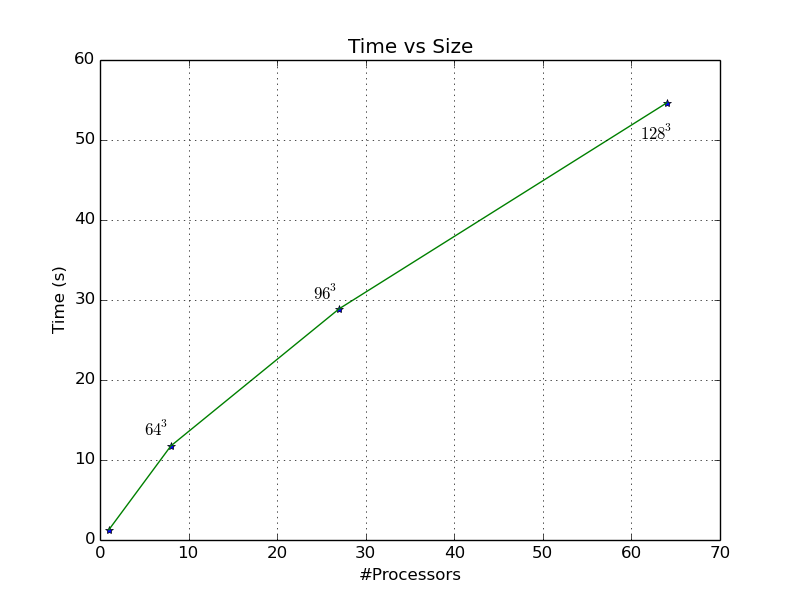
\includegraphics[width = \textwidth]{figures/performance/scalingMG}
		\caption{A Langmuir Oscillation were performed for \(10\) timesteps with a \((32,32,32)\) grid on each processor.
		This was repeated with increasing amount of processors, \((1, 8, 32, 64)\), to see how the multigrid solver scales.}
		% \end{subfigure}
	\end{figure}
	%
	%Comments
	From \cref{sec:para_comp} we expect theoretical optimal scaling of \(\log{N}\log{\varepsilon}\).
	While this was not achieved, the settings were not optimized in these runs, for the various problem sizes and
	this may have caused it to scale worse than it should. When more processors are used the speed of
	the interprocessor communcation may have slowed down, as the processors are not part of the
	same node. The main problem with the test was that the subdomains was very small so
	the communication costs dominated. The communication costs scales linearly \citep{jung_parallelization_1997}, so
	for the coarse grids of the \(5\)-level multigrid the solver scaled close to linearly.

	\citet{baker_scaling_2012} found it crucial to use assumed partition
	to achieve good scalability, as the interprocessor communication costs are the main obstacle to
	scalability for multigrid methods. By assumed partitioning the subdomains are divided into nearby groups
	to easy communication between them.
